\documentclass[10pt]{article}
\usepackage[utf8]{inputenc}
\usepackage[T1]{fontenc}
\usepackage{amsmath}
\usepackage{amsfonts}
\usepackage{amssymb}
\usepackage[version=4]{mhchem}
\usepackage{stmaryrd}
\usepackage{hyperref}
\hypersetup{colorlinks=true, linkcolor=blue, filecolor=magenta, urlcolor=cyan,}
\urlstyle{same}
\usepackage{graphicx}
\usepackage[export]{adjustbox}
\graphicspath{ {./images/} }

\title{Economic shocks and civil conflict at the regional level}


\author{Roland Hodler and Paul Raschky}
\date{}


\begin{document}
\maketitle

\vspace{1cm}

\begin{abstract}

We study the effects of economic shocks on civil conflict at the subnational level using a panel dataset of 5689 administrative regions from 53 African countries with yearly observations from 1992 to 2010.
We find that economic shocks, measured by nighttime light intensity and instrumented by lagged rainfall levels and droughts, increase the probability of civil conflict.

\vspace{0.5cm}

\noindent Keywords: Economic shocks, Civil conflict, Regional development

\noindent JEL classification: C2, D7, O1    

\end{abstract}


\vspace{4cm}


\subsubsection*{Highlights}

\begin{itemize}
  \item We study the effects of economic shocks on civil conflict at the subnational level.

  \item Panel data from 5,689 regions from 53 African countries from 1992 to 2010 are used.

  \item Economic shocks are measured by nighttime light intensity.

  \item Lagged rainfall levels and drought intensity are used as instruments.

  \item Negative economic shocks increase the probability of regional civil conflict.

\end{itemize}

\newpage

\section{Introduction}
In an influential contribution, Miguel et al. (2004) study the effects of economic shocks on civil conflicts in Sub-Saharan Africa. 
They use rainfall patterns to instrument for economic shocks and exploit variation within countries over time to address endogeneity issues and omitted variable bias. 
They find that economic shocks increase the probability of civil conflicts. 
In this letter, we move beyond the country level and exploit variation within subnational regions over time to study the effect of economic shocks, instrumented by rainfall and drought, on civil conflicts at the regional level.


We construct a dataset of 5,689 subnational administrative regions from 53 African countries with yearly observations from 1992 to 2010. 
We thereby rely on the Uppsala Conflict Data Program's Georeferenced Event Dataset (UCDP GED) to construct regional conflict indicators, and on satellite data on nighttime light intensity to measure regional economic activity. 
The use of nighttime light intensity as a measure of economic activity at the subnational level has been forcefully proposed by Henderson et al. (2012).\footnote{Early studies using nighttime light intensity as proxy for economic activity include Sutton and Costanza (2002), Doll et al. (2006), and Sutton et al. (2007). Michalopoulos and Papaioannou $(2013,2014)$ use nighttime light intensity to measure economic activity in a cross-section of African regions, and Hodler and Raschky (2014) in a panel of subnational administrative regions from all over the world}
To instrument for economic activity, we use lagged levels of rainfall inspired by Miguel et al. (2004) and Ciccone (2011), and lagged drought intensity inspired by Couttenier and Soubeyran (2014).

We find that lower levels of rainfall and droughts reduce regional economic activity as proxied by nighttime light intensity in the subsequent period, and, more importantly, that a drop in regional economic activity increases the risk of civil conflict in African regions in the subsequent year. 
A negative economic shock that corresponds to a reduction in the intensity of nightlight by $10 \%$ increases the risk of civil conflict by around 3 percentage points, which corresponds to an increase in this risk from around $4.5 \%$ to around $7.5 \%$ in an average region. 
These results suggest that economic shocks have an important effect on the risk of regional conflict in African regions. 
Hence, the general pattern proposed by Miguel et al. (2004) holds at the more disaggregated level of subnational administrative regions.

There is a large literature on the determinants of civil conflict (see Blattman and Miguel, 2010, for a review). 
We contribute to two strands of this literature. 
First, we contribute to the strand on the causal effects of economic shocks on civil conflict discussed above. 
Second, we contribute to the emerging strand that uses data for subnational regions across Africa, which started with Buhaug and Rod (2006). 
Michalopoulos and Papaioannou (2011), and Besley and Reynal-Querol (2014) focus on how ethnic partitions and historical conflicts affect today's risk of civil conflict. 
Harari and La Ferrara (2013) study the relationship between weather shocks in the growing season of different crops and subsequent civil conflict using subnational regions that are rectangular cells (rather than administrative regions). 
We view their study and ours as complementary. 
They nicely document the impact of weather shocks on civil conflict primarily through agriculture, and our two-stage least squares estimates with the chosen lag structure suggest that the income effect of weather shocks is crucial for their impact on civil conflict. 
Taken together, these two studies imply that weather shocks have a strong impact on civil conflict by changing incomes in the agricultural sectors.

The remainder of this paper is organized as follows: Section 2 presents the data, Section 3 the empirical specification, Section 4 our findings, and Section 5 briefly concludes.

\section{Data}

The Center for International Earth Science Information Network (CIESIN) at Columbia University and its project partners provide information on subnational administrative regions and their boundaries. 
Our units of observation are administrative regions at the second subnational level. 
Our sample consists of 5,689 regions from the 53 African countries for which CIESIN provides the corresponding regional boundaries.\footnote{The following 53 countries are in our sample: Algeria, Angola, Benin, Botswana, Burkina Faso, Burundi, Cameroon, Cape Verde, Central African Republic, Chad, Comoros, Congo (DRC), Congo (RC), Cote d'Ivoire, Djibouti, Egypt, Equatorial Guinea, Eritrea, Ethiopia, Gabon, Gambia, Ghana, Guinea, Guinea-Bissau, Kenya, Lesotho, Liberia, Libya, Madagascar, Malawi, Mali, Mauritania, Mauritius, Morocco, Mozambique, Namibia, Niger, Nigeria, Rwanda, Sao Tome and Principe, Senegal, Sierra Leone, Somalia, South Africa, Sudan, Swaziland, Tanzania, Togo, Tunisia, Uganda, Western Sahara, Zambia, and Zimbabwe.}

Our dependent variables are based on the UCDP GED, which is an event-based and georeferenced dataset on organized violence in Africa between 1989 and 2010. 
For each individual violent event, there is information on the place of the event (with coordinates), the date of the event, the actors participating in the event, and the estimates of fatalities.\footnote{ We employ the UCDP GED rather than the Armed Conflict Location and Event Dataset (ACLED) mainly because the latter only starts in 1997. Moreover, Eck (2012) raises some doubts about the quality of the georeferences in ACLED.} 
Most country-level studies of civil conflict, including Miguel et al. (2004), use as dependent variable a dummy variable that classifies a country-year as having a civil conflict when there are more than 25 conflict-related deaths. 
Given that there are 107 subnational regions in an average country in our sample, we use two different dummy variables: $Conflict01_{i t}$ and $Conflict25_{i t}$, which are equal to one if there are more than one or more than 25 conflict-related deaths, respectively, in region $i$ in year $t$.

Our measure of economic activity is based on satellite data on the intensity of nighttime lights. 
Weather satellites from the US Air Force circle the earth 14 times per day and measure light intensity. 
The National Oceanic and Atmospheric Administration (NOAA) uses observations from evenings during the dark half of the lunar cycle in seasons when the sun sets early, but removes observations that could be affected by, e.g., cloud coverage, fires or other ephemeral lights.
It then provides annual data for the time period from 1992 to 2010 for output pixels that correspond to less than one square kilometer. 
The data comes on a scale from 0 to 63 , with higher values implying more intense nighttime light. 
Henderson et al. (2012) find a high correlation between changes in nighttime light intensity and GDP at the country level, and Hodler and Raschky (2014) document a similar relationship at the level of subnational administrative regions. 
A main advantage of nighttime light intensity is its availability at the regional level, which is particularly useful in the African context where regional GDP estimates are typically poor or unavailable. 
The variable  $Light_{i t}$ corresponds to the logarithm of the average nighttime light intensity of the pixels in region $i$ in year $t$.\footnote{To avoid losing observations with a reported nighttime light intensity of zero, we follow Michalopoulos and Papaioannou $(2013,2014)$, and Hodler and Raschky (2014) in adding $0.01$ to the average nighttime light intensity before taking the logarithm. We do the same when taking the logarithm of average precipitation. Note that our results remain qualitatively and quantitatively similar when excluding all regions in which reported nighttime light intensity is zero throughout the sample period. (Results are available upon request.)}

Following Miguel et al. (2004) and Ciccone (2011), our first instrumental variable is the lagged level of rainfall (in logs).\footnote{Miguel et al. (2004) use lagged year-to-year changes in rainfall, but Ciccone (2011) argues that using the logarithm of lagged levels of rainfall is more appropriate.}
The Climatic Research Unit provides monthly precipitation data on a $0.5 \times 0.5$ degree grid.\footnote{One degree corresponds on average to approximately $110 \mathrm{~km}$.}
The variable Rain $_{i t}$ corresponds to the logarithm of average precipitation in region $i$ in year $t$.

Our second instrumental variable is based on the Palmer Drought Severity Index (PDSI), which combines precipitation, temperature and local soil characteristics. 
Dai et al. (2004) provide monthly PDSI on a $2.5 \times 2.5$ degree grid, with negative values implying dry areas. 
Couttenier and Soubeyran (2014) show that the association between PDSI and conflict is stronger than the one between rainfall and conflict at the country level, and that low PDSI is associated with low crop yields. 
The variable  $Drought_{i t}$ is equal to the average PDSI in region $i$ in year $t$.

Table 1 provides summary statistics for our five main variables.

Table 1: Summary statistics.

\begin{center}
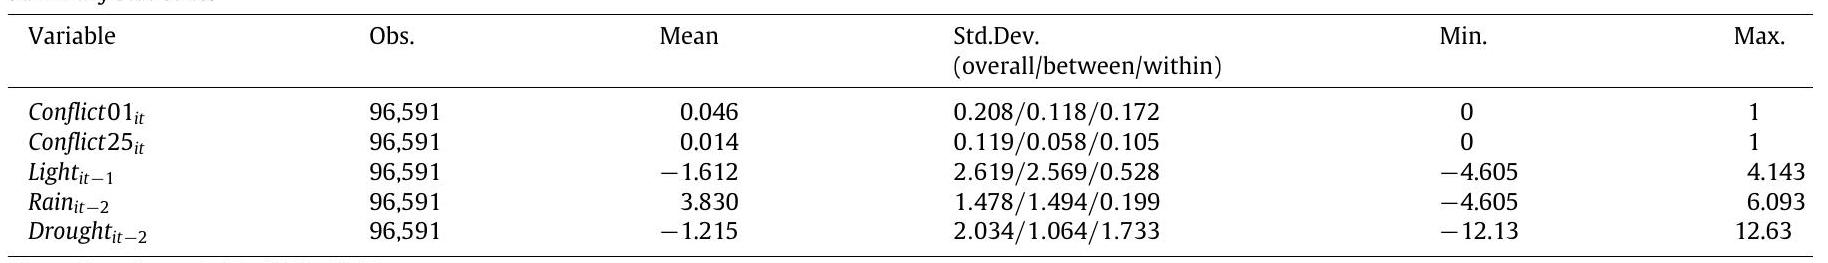
\includegraphics[max width=\textwidth]{2022_11_30_4646cdc62709efe1549cg-3}
\end{center}


\section{Empirical specification}

To estimate the effect of nighttime light intensity on conflict, we start with the following specification:

\begin{equation}
    Conflict_{i t}=\alpha_{i}+\beta_{i} t+\gamma_{t}+\delta Light_{i t-1}+\epsilon_{i t},
\end{equation}
where $Conflict i_{i t}$ is either $Conflict01_{i t}$ or $Conflict 25_{i t}$. 
The regional dummy variables $\alpha_{i}$ and the region-specific time trends $\beta_{i} t$ control for time-invariant regional characteristics, such as size and geography, and for different trends across regions during our sample period. 
The year dummy variables $\gamma_{t}$ control for changes in satellites and their sensor setting as well as global and continent-wide economic and political developments.

 To address endogeneity we follow Miguel et al. (2004) in applying an instrumental variables approach. 
 In the first stage we estimate

\begin{equation}
\text { Light }_{i t-1}=\widetilde{\alpha}_i+\tilde{\beta}_i t+\tilde{\gamma}_t+\tilde{\delta} \text { Weather } r_{i t-2}+\tilde{\epsilon}_{i t}
\end{equation}
where $Weather_{i t}$ can be $Rain_{i t}$ or $Drought_{i t}$. 
In the second stage we estimate specification (1) using the predicted values of $Light_{i t-1}$. 
The exclusion restriction requires that $Weather_{i t-2}$ has no effect on $Conflict _{i t}$ other than through its effects on economic activity and $Light_{i t-1}$. 
It is typically (almost) impossible to establish with certainty that an exclusion restriction holds. 
We however think that our simple and intuitive lag structure makes it quite likely.


Table 2:  Effects on regional conflicts with one or more conflict-related fatalities.

\begin{center}
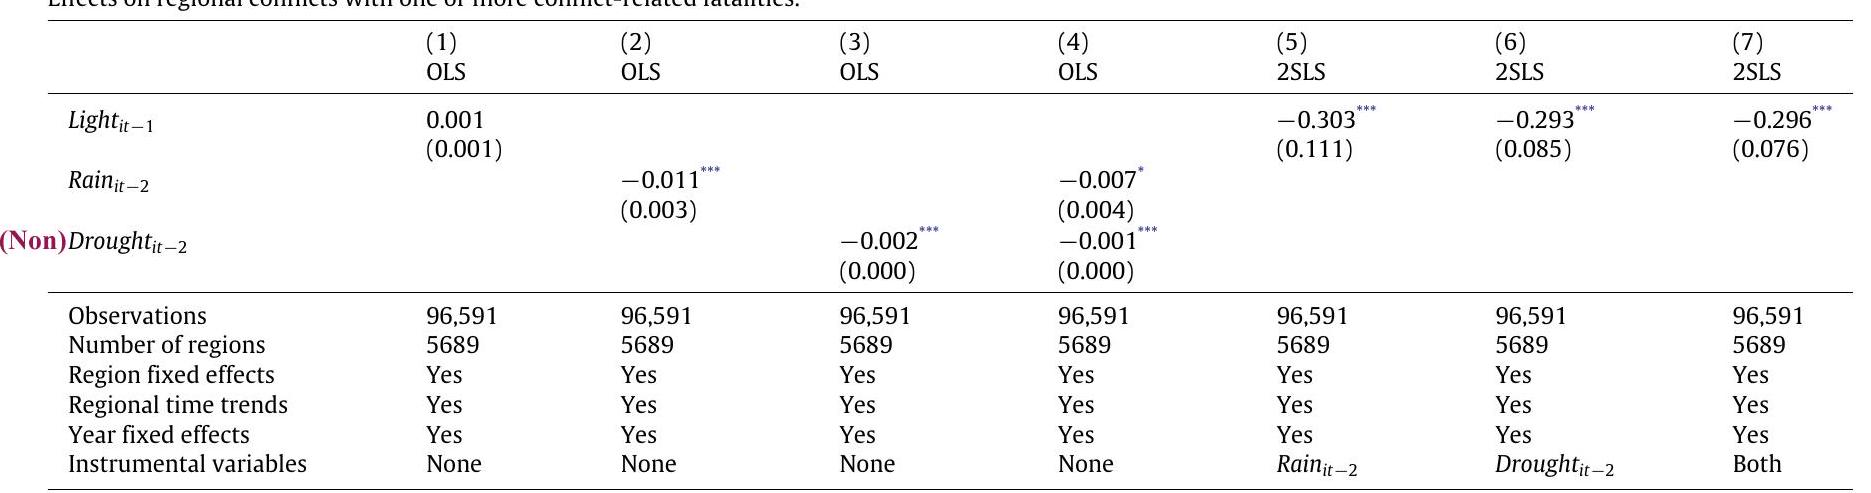
\includegraphics[max width=\textwidth]{2022_11_30_4646cdc62709efe1549cg-3(1)}
\end{center}

Notes: Dependent variable is Conflict $01_{i t}$. Sample period is 1994-2010. Standard errors are adjusted for clustering at the level of administrative regions. Sample period is 1994-2010. Positive values of Drought indicate NON-dry. Indicate significance at the $10 \%$-level. ${ }^{* *}$ Indicate significance at the 5\%-level. Indicate significance at the $1 \%$-level.



\section{Findings}
In Table 2 we analyze the effect of regional economic shocks on all regional conflicts that lead to a least one conflict-related death per year. 
In column 1, we estimate the effect of economic activity on $Conflict01_{i t}$ using a standard OLS regression with region and year fixed effects. 
Lagged economic activity, as measured by $Light_{i c t-1}$, yields a coefficient that is close to zero and not statistically significant. 
In columns 2-4, we present reduced-form estimates in which we directly regress $Conflict01_{i t}$ on our instrumental variables  $Rain_{i t-2}$ and $Drought_{i t-2}$. 
The results indicate that higher rainfall levels and lower drought intensity (i.e., higher PDSI) are associated with fewer regional conflicts in the future. 
In columns 5–7 we present our 2SLS estimates. 
We use  or  or both as instrumental variables for lagged economic activity. 
In all cases, the coefficient on our measure of lagged economic activity, $Light_{i c t-1}$, is negative and statistically significant. 
Hence, there is a considerable difference between our OLS and our 2SLS estimates. 
We think the main reason is that nighttime light intensity is a good, but far from perfect measure of economic activity, and that the instrumental variables approach helps us to address the attenuation bias that can result from the measurement error in the explanatory variables.\footnote{Miguel et al. (2004) also find that the effect of economic shocks on civil conflict is much larger in their 2SLS than their OLS estimates. They think that the main reason is “the problem of measurement error in African national income figures, which are widely thought to be unreliable” (p. 727), and they see the larger 2SLS estimates as an indication that this problem “is likely to be larger than the endogeneity bias, which is presumably negative” (p. 740).}

Table 2: Here

The coefficient estimates are around $-0.3$ in all 2SLS regressions reported in Table 2. 
These estimates suggest that a negative economic shock which decreases nighttime light intensity by $10 \%$, increases the risk of civil conflict with at least one fatality by around 3 percentage points, which corresponds to an increase in this risk from around $4.5 \%$ to around $7.5 \%$ in an average region.

In Table 3,  we analyze the effect of regional economic shocks on larger regional conflicts with 25 or more conflict-related deaths per year. 
The OLS regression in column 1 shows no effect of $Light_{i c t-1}$ on $Conflict25_{i t}$. 
The reduced-form estimates in columns 2-4 again suggest positive effects of $Rain_{i t-2}$ and $Drought_{i t-2}$, but these effects are somewhat weaker than in Table 2. 
The 2SLS regressions in columns 5-7 all yield coefficient estimates around $-0.09$. 
These estimates are statistically significant when using $Drought _{i t-2}$ or both instrumental variables. 
Hence, a negative economic shock which decreases nighttime light intensity by $10 \%$, increases the risk of civil conflict with 25 or more fatalities by almost 1 percentage point, which corresponds to an increase in this risk from around $1.5 \%$ to almost $2.5 \%$ in an average region.

Table 4 contains the first-stage results from our 2SLS regressions. 
The coefficients of  $Rain_{i t-2}$ and $Drought_{i t-2}$ have the expected signs and are statistically significant. 
Higher rainfall levels and lower drought intensity increases economic activity in the subsequent year. 
The first-stage F-stats are above the critical value suggested by Stock and Wright (2000), which is in our case 16.38.


Table 3: Effects on regional conflicts with 25 or more conflict-related fatalities.

\begin{center}
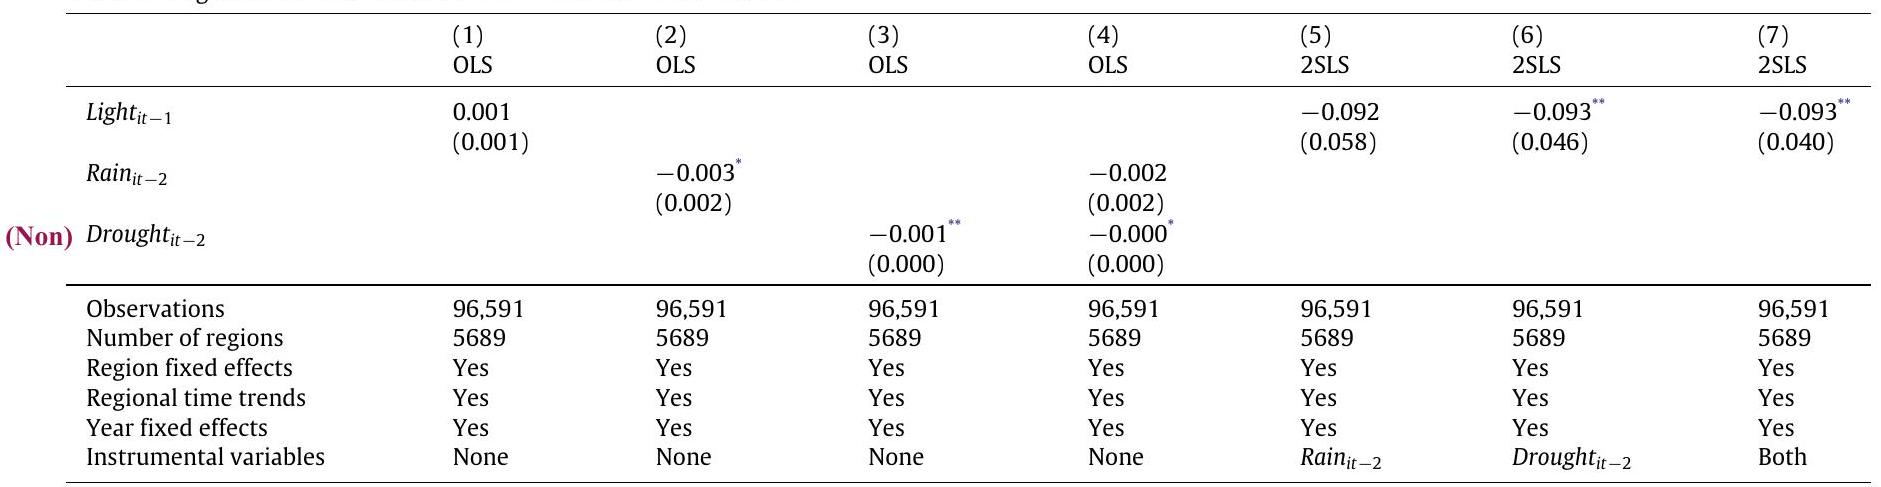
\includegraphics[max width=\textwidth]{2022_11_30_4646cdc62709efe1549cg-4}
\end{center}

Notes: Dependent variable is Conflict $25_{i t}$. Sample period is 1994-2010. Standard errors are adjusted for clustering at the level of administrative regions. Indicate significance at the $10 \%$-level.  Indicate significance at the 5\%-level. *** Indicate significance at the $1 \%$-level.

Table 4: First-stage results.

\begin{center}
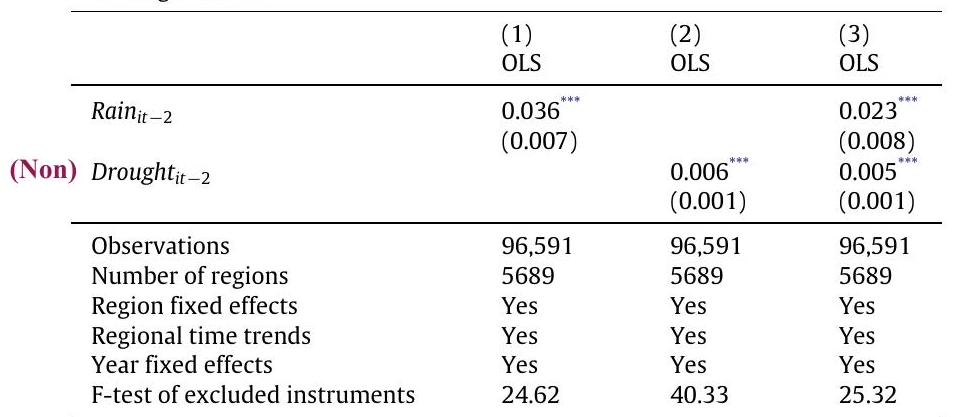
\includegraphics[max width=\textwidth]{2022_11_30_4646cdc62709efe1549cg-4(1)}
\end{center}

Notes: Columns 1-3 report the first-stage estimates of the 2SLS regressions reported in columns 5-7 of Tables 2 and 3. Dependent variables is Light ${ }_{i t-1}$. Sample period is 1994-2010. Standard errors are adjusted for clustering at the level of administrative regions. Indicate significance at the $10 \%$-level. Indicate significance at the $5 \%$-level. Indicate significance at the $1 \%$-level.

\section{Conclusions}
We have taken the seminal contribution of Miguel et al. (2004) to the level of subnational administrative regions, thereby using satellite data on nighttime light intensity to measure economic activity. 
Our results show that regional economic activity has an important effect on the risk of civil conflict in African regions.

\section*{Acknowledgments}
We thank an anonymous referee and conference participants in Lucerne, Passau and Wageningen for helpful comments and the Australian Research Council (ARC DP120103492) for financial support.

\section*{References}
Besley, T.J., Reynal-Querol, M., 2014. The legacy of historical conflict: Evidence from Africa. Amer. Political Sci. Rev. 108 (2), 319-367.

Blattman, C., Miguel, E., 2010. Civil wars. J. Econom. Literature 48 (1), 3-57.

Buhaug, H., Rod, J.K., 2006. Local determinants of African civil wars, 1970-2001. Political Geogr. 25, 315-335.

Ciccone, A., 2011. Economic shocks and civil conflict: A comment. Amer. Econ. J. Appl. Econ. 3 (4), 215-227.

Couttenier, M., Soubeyran, R., 2014. Drought and civil war in sub-Saharan Africa. Econ. J. 124 (575), 201-244.

Dai, A., Trenberth, K.E., Qian, T., 2004. A global data set of Palmer Drought Severity Index for 1870-2002: Relationship with soil moisture and effects of surface warming. J. Hydrometeorology 5, 1117-1130.

Doll, C.N.H., Muller, J.P., Morley, J.G., 2006. Mapping regional economic activity from night-time light satellite imagery. Ecol. Econ. 57 (1), 75-92.

Eck, K., 2012. In data we trust? A comparison of UCDP GED and ACLED conflict events datasets. Cooperation Conflict 47 (1), 124-141.

Harari, M., La Ferrara, E., 2013. Conflict, climate and cells: A disaggregated analysis. CEPR Discussion Paper 9277.

Henderson, V.J., Storeygard, A., Weil, D.N., 2012. Measuring economic growth from outer space. Amer. Econ. Rev. 102 (2), 994-1028.

Hodler, R., Raschky, P.A., 2014. Regional favoritism. Quart. J. Econ. 129 (2), $995-1033$

Michalopoulos, S., Papaioannou, E., 2011. The long-run effects of the scramble for Africa. NBER Working Paper 17620.

Michalopoulos, S., Papaioannou, E., 2013. Pre-colonial ethnic institutions and contemporary African development. Econometrica 81 (1), 113-152.

Michalopoulos, S., Papaioannou, E., 2014. National institutions and subnational development in Africa. Quart. J. Econ. 129 (1), 151-213.

Miguel, E., Satyanath, S., Sergenti, E., 2004. Economic shocks and civil conflict: An instrumental variables approach. J. Political Econ. 112 (4), 725-753.

Stock, J.H., Wright, J.H., 2000. GMM with weak identification. Econometrica 68 (5), $1055-1096$.

Sutton, P.C., Costanza, R., 2002. Global estimates of market and non-market values derived from nighttime satellite imagery, land use, and ecosystem service valuation. Ecol. Econ. 41 (3), 509-527.

Sutton, P.C., Elvidge, C.D., Ghosh, T., 2007. Estimation of gross domestic product at sub-national scales using nighttime satellite imagery. Int. J. Ecol. Econ. Stat. 8 (S07), 5-21.


\end{document}